\documentclass[11pt]{article}

\usepackage[T1]{fontenc}
\usepackage[utf8]{inputenc}
\usepackage{lmodern}
\usepackage{amsmath,amssymb,amsthm,mathtools}
\usepackage{microtype}
\usepackage[margin=0.92in]{geometry}
\usepackage{booktabs,longtable,tabularx,array}
\usepackage{enumitem}
\usepackage{xcolor}
\usepackage{graphicx}
\usepackage{float}
\usepackage{listings}
\usepackage{xurl}
\usepackage{hyperref}

\definecolor{deepblue}{RGB}{28,72,120}
\definecolor{deepgreen}{RGB}{39,108,70}
\definecolor{warmbrown}{RGB}{130,82,25}
\definecolor{codegray}{RGB}{247,247,247}
\definecolor{rulegray}{RGB}{185,185,185}

\hypersetup{
  colorlinks=true,
  linkcolor=deepblue,
  urlcolor=deepblue,
  citecolor=deepgreen,
  pdftitle={Contender 20: Third-Order Autonomous Hyperreflection in BusyLean},
  pdfauthor={BusyLean research proposal},
  pdfsubject={A constructive large-number definition and Lean proof package}
}

\lstdefinelanguage{Lean}{
  morekeywords={
    abbrev,axiom,by,change,class,def,deriving,else,end,exact,export,
    forall,fun,have,if,import,in,inductive,instance,let,match,namespace,
    open,opaque,partial,private,protected,return,structure,termination_by,
    theorem,then,unsafe,where,with
  },
  sensitive=true,
  morecomment=[l]{--},
  morecomment=[s]{/-}{-/},
  morestring=[b]",
}

\lstset{
  language=Lean,
  basicstyle=\ttfamily\footnotesize,
  keywordstyle=\bfseries\color{deepblue},
  commentstyle=\itshape\color{black!58},
  stringstyle=\color{warmbrown},
  backgroundcolor=\color{codegray},
  frame=single,
  framerule=0.35pt,
  rulecolor=\color{rulegray},
  xleftmargin=0.7em,
  xrightmargin=0.7em,
  columns=fullflexible,
  keepspaces=true,
  breaklines=true,
  breakatwhitespace=false,
  showstringspaces=false,
  tabsize=2,
  literate=
    {→}{{$\to$}}1
    {←}{{$\leftarrow$}}1
    {∀}{{$\forall$}}1
    {≤}{{$\le$}}1
    {∧}{{$\wedge$}}1
    {∈}{{$\in$}}1
    {⟨}{{$\langle$}}1
    {⟩}{{$\rangle$}}1
    {·}{{$\cdot$}}1
}

\newtheorem{theorem}{Theorem}[section]
\newtheorem{lemma}[theorem]{Lemma}
\newtheorem{proposition}[theorem]{Proposition}
\newtheorem{corollary}[theorem]{Corollary}
\theoremstyle{definition}
\newtheorem{definition}[theorem]{Definition}
\newtheorem{construction}[theorem]{Construction}
\theoremstyle{remark}
\newtheorem{remark}[theorem]{Remark}
\newtheorem{warning}[theorem]{Validation warning}

\newcommand{\N}{\mathbb{N}}
\newcommand{\Family}{\mathsf{Family}}
\newcommand{\Transformer}{\mathsf{Transformer}}
\newcommand{\TLift}{\mathsf{TransformerLift}}
\newcommand{\LLift}{\mathsf{LiftTransformer}}
\newcommand{\Good}{\mathsf{GoodLift}}
\newcommand{\Progressive}{\mathsf{Progressive}}
\newcommand{\leanname}[1]{\nolinkurl{#1}}
\newcommand{\Cnineteen}{\mathsf{C}_{19}}
\newcommand{\Ctwenty}{\mathsf{C}_{20}}
\newcommand{\Ftwenty}{F_{20}}
\newcommand{\Fnineteen}{F_{19}}
\newcommand{\code}[1]{\texttt{#1}}

\title{\textbf{Contender 20: Third-Order Autonomous Hyperreflection in BusyLean}\\[0.35em]
  \large A constructive large-number definition, domination argument, and Lean integration package}
\author{Research proposal for the BusyLean project}
\date{13 October 2026}

\begin{document}
\maketitle

\begin{abstract}
BusyLean formalizes a ``name the biggest number'' contest in Lean~4: each entry
must be a closed computable natural number, and each improvement must be
accompanied by a formal strict inequality.  At the audited repository head,
Contender~19 combines two powerful components.  Its object language is a
strongly normalizing ladder of universes indexed by Sch\"utte-style
large-Veblen terms, and its amplifier is a natural hierarchy of
\emph{transformer lifts} constructed by diagonal hyperreflection.

This article proposes Contender~20, which raises the amplifier by one explicit
type level.  A new \emph{lift transformer} maps transformer lifts to transformer
lifts.  We define coordinatewise splicing of whole lifts, a promotion operation
that internalizes one successor step of the accepted diagonal hierarchy, a
well-founded tree recursion over lift transformers, an autonomous third-order
closure, and a finite meta-rank iteration of that closure.  Both the schedule
and the two ranks are controlled by the complete Contender~19 family at the
current input.  The resulting lift acts on large-Veblen reflection to produce a
countable family; one final large-Veblen reflection then sees that whole family.
The proposed closed number is
\[
  \Ctwenty = F_{20}(F_{20}(42)).
\]

The comparison architecture is intentionally stronger than the contest's
minimum.  The central invariant \leanname{GoodLift} says that a transformer lift
preserves progressive transformers and is strictly inflationary on them.  It is
preserved by splicing, promotion, tree iteration, autonomous closure, and every
finite meta-rank.  The main architectural theorem states that the final
third-order lift strictly exceeds its entire initial current-style
\leanname{diagonalLift} at every visible coordinate.  Pointwise domination of
the Contender~19 family and a final input-growth argument then yield the required
statement
\[
  \Cnineteen < \Ctwenty.
\]
A second theorem bounds every enumerated large-Veblen-ladder program run
relative to the final packed third-order family.

All definitions are structural recursions on natural numbers or well-founded
W-trees and are computable in principle.  This package includes Lean sources,
a focused axiom/dependency audit, a clean-build timing harness, a guarded
installer, a unified patch, source-provenance data, diagrams, and a compiled
PDF.  The packaging environment did not contain Lean or Lake.  Accordingly,
the article distinguishes source-level evidence from pending Lean~4.34.0 kernel
replay and makes no unverified axiom or timing claim.
\end{abstract}

\tableofcontents
\newpage

%======================================================================
\section{Problem, baseline, and research standard}

The large-number game becomes mathematically substantive when two shortcuts are
forbidden.  First, the proposed number must be computable rather than defined
through an uncomputable extremal function such as Busy Beaver.  Second, a
larger-number claim must be a theorem rather than an informal appeal to a
notation's intended strength.  The original contest of Roux used Coq; BusyLean
ports the game to Lean~4 and has developed a long sequence of successively
stronger reflective constructions~\cite{RouxContest,BusyLeanRepo,Aaronson}.

The package was prepared against the audited BusyLean \code{main} commit
\nolinkurl{64d31a0cf6f1aa4477a088be5554957de6e87a61}.  The pinned toolchain is
\code{leanprover/lean4:v4.34.0}.  At that head, Contender~19 is the accepted
entry.  Its defining equations are, schematically,
\begin{align*}
  \operatorname{family}_{18}(n) &:= F_{18}(F_{18}(n)),\\
  F_{19}(n) &:=
    \operatorname{diagonalLift}(S_{19}(n),r_{19}(n),L,
       \operatorname{family}_{18},n,n),\\
  \Cnineteen &:= F_{19}(F_{19}(42)),
\end{align*}
where $L$ is large-Veblen-ladder reflection, $S_{19}(n)$ is a self-sized
well-founded schedule, and $r_{19}(n)=\operatorname{family}_{18}(n)+1$.

\subsection{Contest constraints}

A proposal intended for integration must satisfy more than mathematical
plausibility.  The current repository rules require the following.

\begin{enumerate}[leftmargin=*,itemsep=0.35em]
\item The entry is a closed, computable Lean \leanname{Nat}.  Definitions using
  \leanname{noncomputable}, \leanname{partial}, \leanname{unsafe}, opaque
  executable stand-ins, foreign implementations, or uncomputable oracles are
  excluded.
\item A theorem proves strict domination of the accepted predecessor.
\item Kernel dependencies are restricted to \leanname{propext} and
  \leanname{Quot.sound}; in particular, \leanname{Classical.choice}, custom
  axioms, \leanname{sorry}, and \leanname{native_decide} are excluded.
\item With earlier contenders precompiled, the new definition is allotted
  15 seconds and the new proof phase 60 seconds on a reasonable machine.
\item The definition may use the predecessor's \emph{construction} as a seed,
  but it may not simply mention the predecessor's closed constant and add or
  iterate something trivial.
\item The kernel, elaborator, and build toolchain may not be exploited.
\end{enumerate}

These constraints shape the mathematics.  A valid improvement needs a total
higher-order construction whose strictness follows from explicit finite
maxima or visible recursive occurrences, rather than from an unproved semantic
monotonicity principle.

\subsection{Meaning of ``significantly exceeds''}

Every legal successor must be strictly larger, but a research-quality proposal
should expose a qualitative increase.  This package adopts the following
standard.

\begin{definition}[Architectural significance]
A successor construction is architecturally significant when it introduces a
new reusable closure principle and proves a strict domination theorem for an
entire predecessor-style operator, not merely for one closed numerical output.
\end{definition}

Contender~20 meets this standard through the theorem
\leanname{diagonalLift_lt_lift20}: at fixed input, its completed third-order
lift dominates a complete current-style diagonal hyperlift instantiated with
the same stronger schedule and inner rank.  The final number comparison is a
corollary of that architecture plus explicit reflection maxima.

\begin{warning}
The Lean code in this archive is a carefully matched proof draft, not a claimed
kernel-checked result.  The packaging environment had no \code{lean} or
\code{lake} executable.  The included \leanname{check20.py} performs the
mandatory replay, axiom closure, dependency closure, and timing tests in a
proper BusyLean checkout.
\end{warning}

%======================================================================
\section{The accepted machinery through Contender 19}

Understanding the proposed increase requires separating the repository's
\emph{object-language axis} from its \emph{amplifier axis}.

\subsection{Families and transformers}

A countable oracle family has two natural-number arguments:
\[
  \Family := \N \to \N \to \N.
\]
The first argument selects an oracle coordinate and the second is the numerical
input.  A transformer maps such families to such families:
\[
  \Transformer := \Family \to \Family.
\]
BusyLean's primitive reflective transformer evaluates a bounded collection of
programs relative to a packed oracle family and returns a number strictly above
all visible oracle values and all bounded program values.  A transformer
$T$ is called progressive when
\[
  i\le n \quad\Longrightarrow\quad
  s(i,n)<T(s)(o,n)
\]
for every seed family $s$ and output coordinate $o$.

The definition is deliberately coordinate-sensitive.  Progressivity is not a
monotonicity assertion of the form $s\le t\Rightarrow T(s)\le T(t)$.  Reflective
programs can inspect and branch on oracle values, so semantic monotonicity is in
general false.  BusyLean's proofs instead track a selected child or a selected
coordinate that literally occurs in the next maximum.

\subsection{Autonomous lifting}

A \emph{transformer lift} acts on transformers:
\[
  \TLift := \Transformer \to \Transformer.
\]
The repository's \leanname{liftTransformer} iterates a progressive transformer
along a universal well-founded W-tree.  Its strictness theorem has the form
\[
  T(s)(i,n)<\operatorname{liftTransformer}(T)(s)(o,n),
  \qquad i\le n.
\]
The proof follows a concrete path through the universal tree.  It does not
compare arbitrary oracles.

The function \leanname{stageLift} accepts an arbitrary transformer lift $A$, a
base transformer $T$, and a W-tree $a$.  At a leaf it applies $A$ to $T$; at a
node it recursively builds one child transformer per branch, splices those
children coordinatewise, and applies $A$ to the splice.  Thus
\leanname{stageLift} raises tree reflection from families to transformers.

\subsection{Diagonal hyperreflection}

For a fixed schedule $S$, the accepted \leanname{diagonalLift} is a natural
hierarchy of transformer lifts:
\begin{align*}
  D^S_0(T) &:= \operatorname{liftTransformer}(T),\\
  D^S_{k+1}(T) &:=
    \operatorname{stageLift}\bigl(D^S_k,D^S_k(T),S\bigr).
\end{align*}
The successor uses the previous rank twice: as the local lift at every schedule
node and as a pre-amplification of the base.  BusyLean proves two crucial
properties for every $k$:

\begin{enumerate}[leftmargin=*]
\item $D^S_k$ preserves progressive transformers;
\item $D^S_k$ is strictly inflationary on every progressive transformer.
\end{enumerate}

The rank is not a cosmetic counter.  The theorem
\leanname{diagonalLift_rank_lt_succ} proves strict increase from rank $k$ to
rank $k+1$ at every visible coordinate.

\subsection{The large-Veblen object language}

The object-language component of Contender~19 is independent of the amplifier.
Its atom order consists of normal Sch\"utte-style Klammersymbole whose Veblen
argument positions are themselves terms.  The repository constructs a universe
for every well-founded atom order and proves strong normalization of the
universe-ladder language.  A bounded evaluator \leanname{lvalue} therefore
returns a natural number for every bounded, type-checked large-Veblen-ladder
program.  The family reflector
\leanname{reflectLFamily} is explicitly larger than

\begin{itemize}[leftmargin=*]
\item every visible family coordinate $s(i,n)$ with $i\le n$; and
\item every value of a bounded large-Veblen-ladder program run relative to the
  packed family $s$.
\end{itemize}

This is the base transformer \leanname{lTransformer}.  Contender~19 applies a
self-ranked diagonal lift to it.  Contender~20 keeps this powerful object
language and raises the amplifier by one more type level.

%======================================================================
\section{Design alternatives and the chosen increase}

Several superficially easy successors were rejected as insufficiently
informative.

\paragraph{Only increase a numeral.}
Replacing a fixed constant by a larger fixed constant, or composing the final
function one additional time, would prove a larger number but add no closure
principle.  It would also violate the spirit of the no-laziness rule.

\paragraph{Only increase the existing rank.}
Setting the diagonal rank to an even larger expression would remain inside the
same natural hierarchy $D^S_k$.  That is a quantitative increase, but it does
not dominate the hierarchy as an operator in a new way.

\paragraph{Only lengthen the ordinal ladder.}
A collapsing-function notation beyond the large Veblen ordinal would be a
valuable future object-language advance, but a correct normal-form system and
well-foundedness proof are substantial projects.  Raw collapsing terms often
admit descending chains unless normality and side conditions are designed with
great care.  A rushed notation would weaken rather than strengthen the formal
package.

\paragraph{Only reseed Contender 19.}
Using $n\mapsto F_{19}(F_{19}(n))$ as a seed is legal and useful, but reseeding
alone does not explain a new amplifier.

\medskip

The chosen construction uses the accepted diagonal lift as its \emph{initial
object}, then treats entire transformer lifts as branchable, spliceable data.
This is exactly the next simple type over the accepted amplifier:
\[
  \LLift := \TLift\to\TLift.
\]
The new closure acts at this level, and only afterward returns to a numerical
family and performs one final object-language reflection.

\begin{figure}[H]
\centering
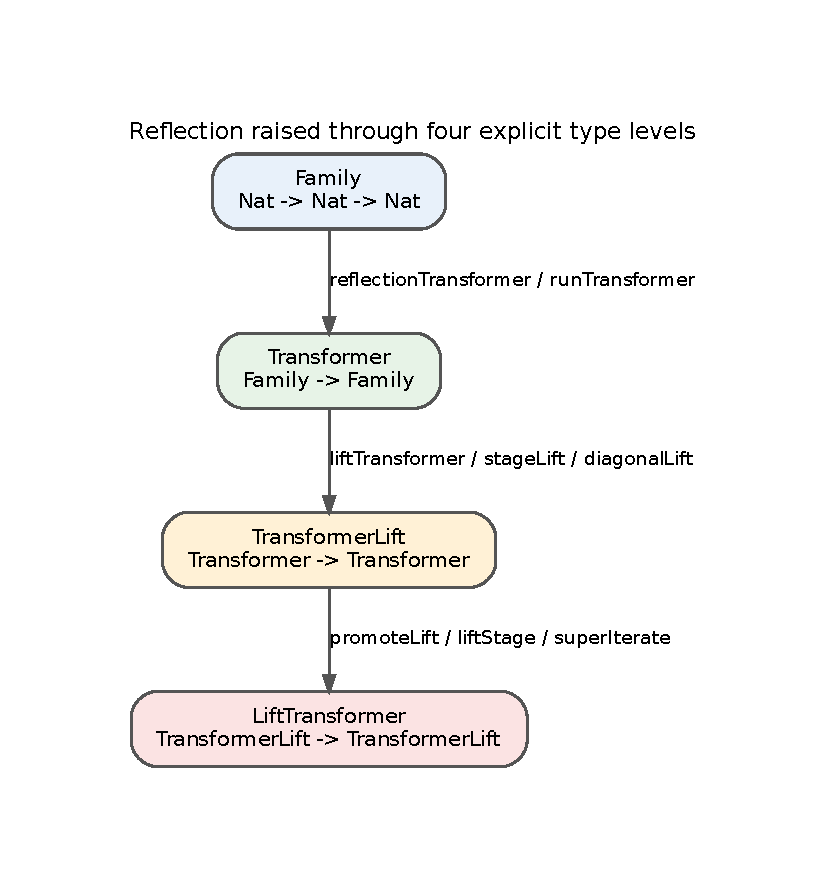
\includegraphics[width=0.76\textwidth]{../artifacts/type_ladder.pdf}
\caption{The new construction raises reflection one explicit simple-type level.
The labels describe Lean abbreviations, not an informal analogy.}
\label{fig:type-ladder}
\end{figure}

%======================================================================
\section{Third-order autonomous hyperreflection}

This section gives the mathematical content of
\leanname{SuperReflection.lean}.  The adjective ``third-order'' refers to the
explicit hierarchy
\[
\begin{gathered}
  \Family,\qquad \Family\to\Family,\qquad
  (\Family\to\Family)\to(\Family\to\Family),\\
  \TLift\to\TLift.
\end{gathered}
\]
It is not a claim about the order of arithmetic or a proof-theoretic ordinal.

\subsection{Splicing whole lifts}

Given a countable family of transformer lifts $A_0,A_1,\ldots$, define a new
lift by
\[
  \operatorname{spliceLifts}(A)(T)
  :=\operatorname{spliceTransformers}(i\mapsto A_i(T)).
\]
At output coordinate $o$, the splice selects $A_o(T)$ and evaluates it at its
canonical output coordinate $0$.  This definition is important for two
reasons.  First, it makes a family of complete amplifiers dynamically
selectable.  Second, it preserves the explicit-coordinate proof discipline:
coordinate $o$ witnesses the occurrence of the $o$th child lift.

\begin{lstlisting}[caption={Coordinatewise splicing at the new type level.}]
abbrev LiftTransformer := TransformerLift → TransformerLift

def spliceLifts (lifts : Nat → TransformerLift) : TransformerLift :=
  fun base => spliceTransformers (fun i => lifts i base)
\end{lstlisting}

\subsection{Promotion internalizes one diagonal successor}

For a fixed schedule $S$, define
\[
  \operatorname{promoteLift}_S(A)(T)
  :=\operatorname{stageLift}(A,A(T),S).
\]
This is precisely the shape of one successor in the accepted diagonal
hierarchy, but abstracted as an operation on arbitrary lifts.  If $A=D^S_k$,
then promotion recovers $D^S_{k+1}$ extensionally at the defining equation.
The abstraction is what allows the successor operation itself to be iterated
along a W-tree.

\begin{lstlisting}[caption={One accepted hyperreflection successor, abstracted as a lift transformer.}]
def promoteLift (schedule : WTree Nat) : LiftTransformer :=
  fun lift base => stageLift lift (lift base) schedule
\end{lstlisting}

\subsection{Tree recursion over lift transformers}

Let $M:\LLift$ and $A:\TLift$.  Define
$\operatorname{liftStage}(M,A,a)$ by recursion on a W-tree $a$:
\begin{align*}
 \operatorname{liftStage}(M,A,\mathsf{leaf})
   &:= M(A),\\
 \operatorname{liftStage}(M,A,\mathsf{node}(f))
   &:=M\left(\operatorname{spliceLifts}
       \bigl(i\mapsto\operatorname{liftStage}(M,A,f(i))\bigr)\right).
\end{align*}
This is the exact next-type analogue of \leanname{stageLift}.  The tree does not
merely choose numbers or transformers; its branches contain complete
transformer lifts.

\begin{lstlisting}[caption={Well-founded tree reflection over complete transformer lifts.}]
def liftStage (amp : LiftTransformer) (base : TransformerLift) :
    WTree Nat → TransformerLift
  | .leaf => amp base
  | .node f =>
      amp (spliceLifts (fun i => liftStage amp base (f i)))
\end{lstlisting}

\subsection{Autonomous closure and finite meta-rank}

The autonomous closure uses the same schedule in two roles:
\[
  \operatorname{superClosure}_S(A)
  :=\operatorname{liftStage}(\operatorname{promoteLift}_S,A,S).
\]
Internally, each application of \leanname{promoteLift} traverses $S$ through
\leanname{stageLift}; externally, \leanname{liftStage} branches over whole lifts
along $S$ again.  This is a genuine nested closure, not a second name for one
rank increment.

Finally define finite iteration:
\begin{align*}
  \operatorname{superIterate}_S(0,A)&:=A,\\
  \operatorname{superIterate}_S(k+1,A)&:=
    \operatorname{superClosure}_S(
       \operatorname{superIterate}_S(k,A)).
\end{align*}
The recursion parameter is a natural number.  Therefore the operation remains
total and executable in principle even when the chosen rank is unimaginably
large.

\begin{lstlisting}[caption={Autonomous third-order closure and its finite meta-rank hierarchy.}]
def superClosure (schedule : WTree Nat) (base : TransformerLift) :
    TransformerLift :=
  liftStage (promoteLift schedule) base schedule

def superIterate (schedule : WTree Nat) :
    Nat → TransformerLift → TransformerLift
  | 0, base => base
  | k + 1, base => superClosure schedule (superIterate schedule k base)
\end{lstlisting}

%======================================================================
\section{The invariant that makes comparison possible}

Higher-order reflection is easy to define and easy to overclaim.  The central
technical contribution is a small invariant strong enough to propagate through
every new constructor and weak enough to be proved without false monotonicity.

\subsection{Two accepted properties}

For a transformer lift $A:\TLift$, BusyLean already defines:

\begin{definition}[Preservation]
$A$ preserves progressivity if every progressive transformer $T$ is mapped to a
progressive transformer $A(T)$.
\end{definition}

\begin{definition}[Strict inflationarity]
$A$ is strictly inflationary if, whenever $T$ is progressive and $i\le n$,
\[
  T(s)(i,n)<A(T)(s)(o,n)
\]
for every family $s$ and output coordinate $o$.
\end{definition}

We package them.

\begin{definition}[Good lift]
\[
  \Good(A) :\Longleftrightarrow
  \operatorname{PreservesProgressive}(A)
  \wedge \operatorname{StrictlyInflationary}(A).
\]
\end{definition}

A lift transformer $M:\LLift$ preserves good lifts when
$\Good(A)\Rightarrow\Good(M(A))$.  It is lift-strict when, for every good $A$
and every progressive $T$,
\[
  A(T)(s)(i,n)<M(A)(T)(s)(o,n)
  \qquad(i\le n).
\]

\subsection{Splicing preserves the invariant}

\begin{lemma}[\leanname{spliceLifts_good}]
If every $A_j$ is a good lift, then
$\operatorname{spliceLifts}(j\mapsto A_j)$ is a good lift.
\end{lemma}

\begin{proof}[Proof idea]
For preservation, fix a progressive base transformer $T$.  Every $A_j(T)$ is
progressive, and the accepted theorem \leanname{spliceTransformers_progressive}
then applies.  For strictness, output coordinate $o$ of the splice is
definitionally coordinate $0$ of $A_o(T)$.  Apply strictness of $A_o$ to the
visible seed coordinate $i$.  No comparison between different seed families is
needed.
\end{proof}

\subsection{Promotion is good and lift-strict}

\begin{lemma}[\leanname{promoteLift_good}]
For every schedule $S$, if $A$ is good, then
$\operatorname{promoteLift}_S(A)$ is good.
\end{lemma}

\begin{proof}[Proof idea]
Preservation is the accepted theorem \leanname{stageLift_progressive}, applied
to the progressive transformer $A(T)$.  For strictness, chain two explicit
inequalities:
\[
  T(s)(i,n)
  < A(T)(s)(i,n)
  < \operatorname{stageLift}(A,A(T),S)(s)(o,n).
\]
The first is strict inflationarity of $A$; the second is the accepted
\leanname{base_lt_stageLift} theorem, with base transformer $A(T)$.
\end{proof}

\begin{lemma}[\leanname{lift_lt_promoteLift}]
If $A$ is good and $T$ is progressive, then
\[
 A(T)(s)(i,n)<\operatorname{promoteLift}_S(A)(T)(s)(o,n)
\]
for every $i\le n$.
\end{lemma}

This second statement is stronger than what is required to show that promotion
is good: it says promotion strictly exceeds the input lift itself.  It becomes
the local strictness hypothesis for the next tree recursion.

\subsection{The node argument one level higher}

\begin{theorem}[\leanname{baseLift_lt_liftStage}]
Suppose $M$ preserves good lifts and is lift-strict.  If $A$ is good and $T$ is
progressive, then for every W-tree $a$ and every visible coordinate $i\le n$,
\[
  A(T)(s)(i,n)
  <\operatorname{liftStage}(M,A,a)(T)(s)(o,n).
\]
\end{theorem}

\begin{proof}[Proof architecture]
At a leaf, this is exactly lift-strictness of $M$.

At a node $\mathsf{node}(f)$, first follow child zero recursively:
\[
  A(T)(s)(i,n)
  <\operatorname{liftStage}(M,A,f(0))(T)(s)(0,n).
\]
By the preceding preservation theorem, every child lift is good, so their
coordinatewise splice is good.  The value of child zero at output coordinate
zero is definitionally coordinate zero of that splice.  Lift-strictness of $M$
therefore gives
\[
 \operatorname{liftStage}(M,A,f(0))(T)(s)(0,n)
 < M(\operatorname{spliceLifts}(\ldots))(T)(s)(o,n),
\]
which is the parent value.  Transitivity completes the proof.

The argument is notable for what it does \emph{not} use: no transitivity of an
ordinal notation order, no monotonicity of program evaluation in an oracle,
and no global comparison of branch families.  Only an explicitly selected
child and an explicitly selected coordinate are used.
\end{proof}

\subsection{Closure and meta-rank growth}

Specializing $M$ to $\operatorname{promoteLift}_S$ yields the following.

\begin{theorem}[Autonomous closure]
If $A$ is good, then $\operatorname{superClosure}_S(A)$ is good and strictly
exceeds $A$ on every progressive base transformer and every visible coordinate.
\end{theorem}

Natural-number induction then gives:

\begin{theorem}[\leanname{superIterate_good}]
For every $k$, if $A$ is good, then
$\operatorname{superIterate}_S(k,A)$ is good.
\end{theorem}

\begin{theorem}[\leanname{superIterate_step_lt}]
For every $k$, progressive $T$, and visible coordinate $i\le n$,
\[
 \operatorname{superIterate}_S(k,A)(T)(s)(i,n)
 <\operatorname{superIterate}_S(k+1,A)(T)(s)(o,n).
\]
\end{theorem}

\begin{corollary}[\leanname{lift_lt_superIterate_succ}]
Every positive meta-rank strictly exceeds the initial lift $A$.
\end{corollary}

This corollary is the formal reason the new meta-rank is extensionally
meaningful.  It is also the bridge to the architectural domination theorem for
Contender~20.

%======================================================================
\section{The exact Contender 20 definition}

The new construction uses the accepted family, but not the accepted closed
constant.

\subsection{The predecessor family}

Define
\[
  \operatorname{family}_{19}(n):=F_{19}(F_{19}(n)).
\]
At $n=42$ this is definitionally Contender~19, but as a function it is available
at every input.  The seed family repeats it at every coordinate:
\[
  \operatorname{seed}_{19}(i,n):=\operatorname{family}_{19}(n).
\]
Using the preceding construction as a family rather than importing the closed
constant follows the established BusyLean pattern and satisfies the no-laziness
rule.

\subsection{A self-sized schedule and two self-sized ranks}

Let
\[
  S_{20}(n)
  :=\operatorname{realize}\!
     \left(\operatorname{hyper}
       (\operatorname{family}_{19}(n)+42,
        \operatorname{encode}(\operatorname{tree}_{12}))\right).
\]
This is a computable W-tree.  Define both ranks by
\[
  r_{\mathrm{in}}(n)=r_{\mathrm{meta}}(n)
  :=\operatorname{family}_{19}(n)+1.
\]
Keeping the two names separate is deliberate.  The inner rank belongs to the
accepted diagonal hierarchy; the meta-rank counts autonomous closures of whole
lifts.  Future variants may separate their growth rates.

\subsection{Initial lift, third-order lift, and final family}

The initial lift is
\[
  A_n:=\operatorname{diagonalLift}(S_{20}(n),r_{\mathrm{in}}(n)).
\]
The third-order lift is
\[
  L_{20}(n):=
  \operatorname{superIterate}
    (S_{20}(n),r_{\mathrm{meta}}(n),A_n).
\]
Applying this lift to the large-Veblen transformer $L$ and the seed family gives
an entire output family:
\[
  H_{20}(n):=L_{20}(n)(L)(\operatorname{seed}_{19}).
\]
In Lean, $H_{20}(n)$ has type \leanname{Family}; it is not prematurely
collapsed to one selected output coordinate.

\subsection{Final reflection and closed number}

The numerical function is a final large-Veblen reflection over the complete
third-order family:
\[
  F_{20}(n):=\operatorname{reflectLFamily}(H_{20}(n),n).
\]
Finally,
\[
  \boxed{\Ctwenty:=F_{20}(F_{20}(42)).}
\]

\begin{lstlisting}[caption={The complete numerical definition.}]
def family19 (n : Nat) : Nat := F19 (F19 n)

def seed19 : Family := fun _ => family19

def schedule20 (n : Nat) : WTree Nat :=
  Autonomous.realize
    (Autonomous.hyper (family19 n + 42) (Autonomous.encode tree12))

def innerRank20 (n : Nat) : Nat := family19 n + 1

def metaRank20 (n : Nat) : Nat := family19 n + 1

def lift20 (n : Nat) : TransformerLift :=
  superIterate (schedule20 n) (metaRank20 n)
    (diagonalLift (schedule20 n) (innerRank20 n))

def hyperFamily20 (n : Nat) : Family :=
  lift20 n lTransformer seed19

def F20 (n : Nat) : Nat :=
  reflectLFamily (hyperFamily20 n) n

def contender_20 : Nat := F20 (F20 42)
\end{lstlisting}

\begin{figure}[H]
\centering
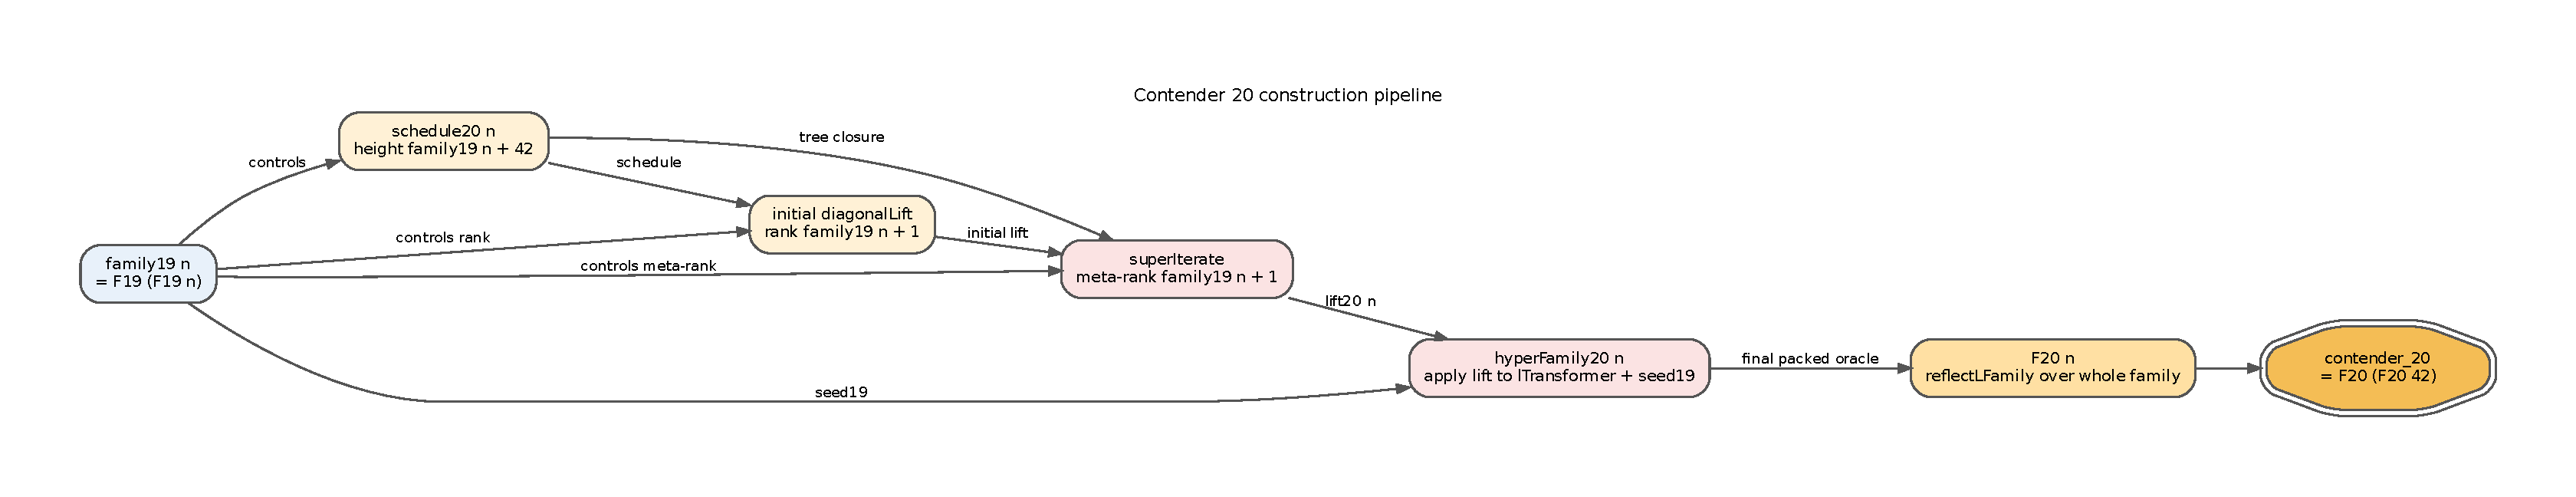
\includegraphics[width=0.99\textwidth]{../artifacts/construction_pipeline.pdf}
\caption{The construction deliberately preserves the complete third-order
family until the final object-language reflection.}
\label{fig:pipeline}
\end{figure}

%======================================================================
\section{Formal domination chain}

The proposed proof has two levels: a reusable operator theorem and the closed
number theorem required by the contest.

\subsection{The initial diagonal lift is good}

The accepted theorems immediately give
\[
  \Good(A_n).
\]
In Lean this is \leanname{diagonalLift20_good}, a pair consisting of
\leanname{diagonalLift_preservesProgressive} and
\leanname{diagonalLift_strictlyInflationary}.  Applying
\leanname{superIterate_good} then gives $\Good(L_{20}(n))$.

\subsection{Architectural domination}

Because $r_{\mathrm{meta}}(n)=\operatorname{family}_{19}(n)+1$ is positive,
\leanname{lift_lt_superIterate_succ} yields the main theorem.

\begin{theorem}[\leanname{diagonalLift_lt_lift20}]
For every input $n$, progressive transformer $T$, seed family $s$, and
$i\le n$,
\[
 A_n(T)(s)(i,n)<L_{20}(n)(T)(s)(o,n).
\]
\end{theorem}

This theorem compares complete lifts under arbitrary progressive bases and
arbitrary seed families.  It does not merely compare the two closed contenders.
Moreover, $A_n$ is a current-style diagonal lift using the \emph{stronger}
Contender~20 schedule and the \emph{stronger} Contender~20 inner rank.  The new
meta-layer strictly exceeds that whole object before the final reflection.

\subsection{The predecessor family is beaten inside the hyper-family}

Since $L_{20}(n)$ preserves progressivity and \leanname{lTransformer} is
progressive, the output transformer
$L_{20}(n)(L)$ is progressive, where $L$ is \leanname{lTransformer}.  Apply it to
\leanname{seed19} and select input coordinate zero:
\[
  \operatorname{family}_{19}(n)
  =\operatorname{seed}_{19}(0,n)
  <H_{20}(n)(0,n).
\]
This is \leanname{family19_lt_hyperFamily20}.

The final reflector contains an explicit prefix maximum over the visible
coordinates of $H_{20}(n)$.  Hence
\[
  H_{20}(n)(0,n)<F_{20}(n).
\]
Combining the two inequalities gives the pointwise theorem
\begin{equation}
  \operatorname{family}_{19}(n)<F_{20}(n).
  \label{eq:family-domination}
\end{equation}

\subsection{The old raw reflection is also below the new family}

Strict inflationarity of $L_{20}(n)$, with base transformer
\leanname{lTransformer}, gives
\[
  \operatorname{reflectLFamily}(\operatorname{seed}_{19},n)
  <H_{20}(n)(0,n).
\]
The final reflection then gives
\[
  \operatorname{reflectLFamily}(\operatorname{seed}_{19},n)<F_{20}(n).
\]
This is useful evidence that the increase is not obtained solely by changing
the seed: even one complete large-Veblen reflection over the old seed lies
strictly below the new third-order family before the final reflection.

\subsection{Programs relative to the final family}

The final layer was chosen so that the strongest program bound concerns the
final oracle family, not merely the old seed.

\begin{theorem}[\leanname{final_lvalue_lt_F20}]
If $t$ is an enumerated large-Veblen-ladder program of depth at most $n$, then
\[
  \operatorname{lvalue}
     (\operatorname{packFamily}(H_{20}(n)),n,t)
  <F_{20}(n).
\]
\end{theorem}

The proof is direct from the maximum built into
\leanname{reflectLFamily}.  It states that the object language may inspect the
complete third-order family through the computable family packing, yet every
bounded program value remains below the final output.

\subsection{The closed comparison}

The accepted input-growth theorem gives
\[
  n<F_{19}(n)<F_{19}(F_{19}(n))
  =\operatorname{family}_{19}(n).
\]
Together with Equation~\eqref{eq:family-domination}, this gives $n<F_{20}(n)$.
Now set $n=42$ in the family domination theorem:
\[
  \Cnineteen
  =\operatorname{family}_{19}(42)
  <F_{20}(42).
\]
Apply input growth at $F_{20}(42)$:
\[
  F_{20}(42)<F_{20}(F_{20}(42))=\Ctwenty.
\]
By transitivity:

\begin{theorem}[Required comparison]
\[
  \boxed{\Cnineteen<\Ctwenty.}
\]
The corresponding Lean declaration is
\leanname{contender_19_lt_contender_20}.
\end{theorem}

%======================================================================
\section{Constructivity and executability}

The values in this contest are intentionally infeasible to evaluate.  That is
not a defect: computability means that a finite procedure exists, not that the
procedure terminates within physical resources.  The proposed definition is
computable for the following concrete reasons.

\subsection{Only structural recursion is introduced}

The new executable definitions recurse on exactly two inductive objects.

\begin{itemize}[leftmargin=*]
\item \leanname{liftStage} recurses structurally on a value of type
  \leanname{WTree Nat}.  Every recursive call is made on an immediate child.
\item \leanname{superIterate} recurses structurally on a natural-number rank.
  The successor case calls the function at the predecessor rank.
\end{itemize}

The schedule itself is produced by the existing computable
\leanname{Autonomous.realize}.  The large-Veblen evaluator uses the existing
strong-normalization proof to define a total normalizer.  The final reflector
uses maxima over finite bounded enumerations.  No semantic search for a proof or
halting witness appears in the executable path.

\subsection{No new axiom is needed by design}

The new definitions are axiom-free executable terms.  The proofs are assembled
from accepted progressivity and strictness theorems, induction, definitional
reduction, and transitivity of natural-number order.  Therefore no use of
choice is mathematically expected.  Nonetheless, Lean's actual dependency
closure is the authority; \leanname{Audit20.lean} prints the axiom sets of the
new key declarations, and \leanname{check20.py} rejects every axiom outside
\leanname{propext} and \leanname{Quot.sound}.

\subsection{The no-laziness condition}

The source definition of \leanname{contender_20} does not mention the constant
\leanname{contender_19}.  It imports and uses $F_{19}$, the previous
construction, to define a seed function at arbitrary inputs.  This is precisely
the distinction allowed by the contest rules.  The focused audit additionally
checks the transitive constant closure of \leanname{contender_20} against all
earlier contender constants.

\subsection{Why the number should never be evaluated}

Even very small fragments of the object-language enumerations grow rapidly, and
the proposed rank is itself controlled by a twice-iterated predecessor family.
Actual evaluation would attempt to realize nested W-tree schedules, repeated
higher-order closures, and bounded normalizations at impossible sizes.  Lean
needs only to type-check the definitions and proofs; it does not normalize the
closed natural number.  The package therefore contains no \code{\#eval} of
any contender.

%======================================================================
\section{Why the increase is substantial}

The strict inequality theorem alone does not communicate the construction's
scale.  Four structural features distinguish Contender~20 from a cosmetic
successor.

\subsection{A new reusable type-level closure}

Contender~19 chooses a large natural rank in a hierarchy of transformer lifts.
Contender~20 makes transformer lifts themselves the branch objects of a
well-founded reflection.  A node can splice a countable family of complete
lifts, and the next operation can inspect that splice as one lift.  This
capability cannot be represented by merely increasing the natural rank of one
fixed \leanname{diagonalLift} definition without inlining a new higher-order
recursion.

\subsection{The accepted hierarchy becomes the base object}

The initial object $A_n$ is not rank zero or a weak primitive.  It is already a
self-ranked current-style diagonal lift with rank
$\operatorname{family}_{19}(n)+1$ and schedule height controlled by the same
predecessor family.  The positive meta-rank then strictly dominates this entire
initial object.

\subsection{The schedule is used at two nested levels}

Within each promotion, \leanname{stageLift} traverses $S_{20}(n)$.  Around those
promotions, \leanname{liftStage} traverses the same schedule while branching
over whole lifts.  Thus each autonomous closure nests schedule-driven
reflection rather than repeating a fixed unary operation.

\subsection{The final object language sees the whole generated family}

The third-order lift is not immediately sampled at one coordinate.  It produces
$H_{20}(n):\Family$, which is packed as the oracle of one final
large-Veblen-ladder reflection.  The final program bound therefore includes
programs that dynamically query coordinates of the generated third-order
family.  This interaction between amplifier and object language is stronger
than appending an arithmetic successor to the amplified value.

%======================================================================
\section{Heuristic growth discussion, with explicit limits}

Fast-growing-hierarchy notation is useful for orientation, but it can be
misleading when a construction mixes impredicative type systems, autonomous
tree reflection, universe ladders, and higher-type operator closure.  The
formal result of this package is a collection of natural-number inequalities,
not an exact ordinal calibration.

\subsection{What can be said safely}

At a qualitative level, the accepted hierarchy
$k\mapsto D^S_k$ is converted from a parameterized family of lifts into the
input of a new autonomous closure operator.  One application of
\leanname{superClosure} contains:

\begin{enumerate}[leftmargin=*]
\item an outer traversal of $S$ whose branches are complete transformer lifts;
\item coordinatewise splicing of those lift branches;
\item at each outer node, a promotion that itself performs an inner
  \leanname{stageLift} traversal of $S$; and
\item pre-amplification of every base transformer by the local lift.
\end{enumerate}

Then this closure is iterated through a rank controlled by the full predecessor
family, and the resulting family is reflected once more by the large-Veblen
object language.  This is compelling structural evidence of a large gap beyond
Contender~19, in addition to the formal strict inequality.

\subsection{What is not claimed}

This article does not identify a proof-theoretic ordinal $\alpha$ such that
$F_{20}$ is equivalent to a standard fast-growing function $f_\alpha$.  It does
not claim that one higher simple type automatically corresponds to a particular
ordinal operation.  It does not compare the construction with arbitrary future
collapsing-function ladders.  Such statements would require a semantic ordinal
analysis of the exact reflective languages and higher operators, not merely an
inspection of source syntax.

The distinction follows the methodological lesson of transfinite reflection
progressions: iteration principles can be calibrated only after the underlying
theory, notation system, fundamental sequences, and reflection schema are
specified precisely~\cite{Feferman1962,Schuette1977,Buchholz1986}.  Here the
kernel-checked inequalities are precise; the scale discussion remains a
research heuristic.

%======================================================================
\section{Lean engineering and replay plan}

The package is organized as an overlay so it can be reviewed without modifying
the repository prematurely.

\subsection{Modules}

\begin{longtable}{>{\raggedright\arraybackslash}p{0.34\textwidth}
                  >{\raggedright\arraybackslash}p{0.60\textwidth}}
\toprule
File & Purpose\\
\midrule
\endfirsthead
\toprule
File & Purpose\\
\midrule
\endhead
\leanname{BusyLean/SuperReflection.lean}
  & New executable type-level operations: \leanname{LiftTransformer},
    \leanname{spliceLifts}, \leanname{promoteLift}, \leanname{liftStage},
    \leanname{superClosure}, and \leanname{superIterate}.\\
\leanname{BusyLean/SuperReflectionFacts.lean}
  & The \leanname{GoodLift} invariant, preservation and strictness lemmas,
    tree-node comparison, and meta-rank growth.\\
\leanname{BusyLean/Contender20.lean}
  & The self-sized schedule, inner and meta ranks, final family, $F_{20}$, and
    the closed number.\\
\leanname{BusyLean/Comparison20.lean}
  & Architectural domination, pointwise family domination, program bound,
    input growth, and the required closed comparison.\\
\leanname{test/Audit20.lean}
  & Focused \code{\#print axioms}, transitive constant-closure rejection,
    and declaration checks.\\
\leanname{scripts/check20.py}
  & Clean build, 15/60-second budget checks, audit execution, and axiom parser.\\
\bottomrule
\end{longtable}

\subsection{Automated acceptance sequence}

After applying the overlay, the intended command is
\begin{lstlisting}[language={},basicstyle=\ttfamily\small]
python3 scripts/check20.py
\end{lstlisting}
It performs the following phases from deleted build directories.

\begin{enumerate}[leftmargin=*]
\item Build \leanname{BusyLean.Comparison19} as the accepted, uncharged
  baseline.
\item Build \leanname{BusyLean.Contender20} and reject a time above 15 seconds.
\item Build \leanname{BusyLean.Comparison20} and reject a time above 60 seconds.
\item Run \leanname{test/Audit20.lean}.
\item Parse all \code{\#print axioms} reports and reject any axiom outside
  the permitted pair.
\item Reject the build if the constant closure of \leanname{contender_20}
  contains any earlier contender constant.
\end{enumerate}

\subsection{Likely elaboration pressure points}

Although the proof draft mirrors accepted signatures, honest engineering
requires identifying where replay may expose a mismatch.

\begin{enumerate}[leftmargin=*]
\item The \leanname{change} step in the node case relies on definitional
  reduction of \leanname{spliceLifts} and \leanname{spliceTransformers} at
  coordinate zero.  If elaboration does not unfold far enough, a local
  \leanname{simpa [spliceLifts, spliceTransformers]} should repair the step
  without changing the theorem.
\item The final comparison relies on definitional equality between
  \leanname{family19 42} and \leanname{contender_19}.  A replay may request an
  explicit \leanname{simpa [family19, contender_19, contender_20]}.
\item Natural-number expressions $(k+1)+1$ and $(\operatorname{succ} k)+1$ are
  definitionally close but may require a one-line simplification in the
  induction on positive meta-ranks.
\item The definition budget should be comfortable because the new executable
  modules are small and predecessor modules are precompiled, but only the
  target machine can establish the timing result.
\end{enumerate}

These are ordinary elaboration risks, not gaps in the mathematical strategy.
The package records them so that any repair remains minimal and auditable.

%======================================================================
\section{Static audit and evidence discipline}

A source audit cannot replace the kernel, but it can prevent avoidable
submission errors.  The included \leanname{static_audit.py} strips nested Lean
comments and strings, then checks the four library modules for forbidden
implementation words and elaboration-time commands.  It checks expected
declarations, verifies that every line is at most 100 columns, confirms that the
definition source contains $F_{19}$ but not the closed constant
\leanname{contender_19}, and records SHA-256 hashes.

The audit report is intentionally labeled
\code{static\_source\_audit\_not\_kernel\_replay}.  It reports
\code{kernel\_replay\_performed: false}.  The claim matrix classifies each
statement as one of:

\begin{itemize}[leftmargin=*]
\item verified by source or PDF tooling;
\item proof drafted but kernel replay pending;
\item entirely unverified until timing or axiom audit runs.
\end{itemize}

This distinction is part of the research result.  Large-number proposals are
particularly vulnerable to impressive notation masking an unchecked premise.
The archive therefore does not convert a missing toolchain into an implicit
claim of success.

%======================================================================
\section{Further research directions}

The proposal opens several concrete lines of work.

\subsection{Generic higher-type reflection towers}

The progression
\[
 \Family,
 \quad \Family\to\Family,
 \quad \TLift,
 \quad \LLift
\]
can be abstracted using an indexed family of simple types and a generic notion
of coordinatewise splicing.  One could define a finite tower whose height is
itself input-controlled.  The main challenge is not the executable recursion
but a uniform invariant that specializes to progressivity and strict
inflationarity at each level without generating unmanageable dependent casts.

\subsection{Well-founded rather than finite meta-ranks}

The accepted repository already builds universe ladders over arbitrary
well-founded atom orders.  A natural next question is whether
\leanname{superIterate} can be generalized from $\N$ to an explicit
well-founded notation type.  At a limit notation, the operation would need to
splice the lower-rank lifts in a way that preserves \leanname{GoodLift}.  The
current \leanname{spliceLifts_good} theorem is exactly the local lemma such a
construction would require.  A meaningful proposal would need an explicit
fundamental-sequence or predecessor enumeration and a strict comparison theorem
for every accessible notation.

\subsection{Collapsing-function atom orders}

The object-language axis can be advanced independently.  Extending the ladder
beyond the large Veblen ordinal with Buchholz-style or Takeuti-style collapsing
functions is attractive, but raw terms are not automatically well-founded
under the intended comparison.  The research task is to design normal forms,
side conditions, and a Boolean comparison whose case split supports a Lean
accessibility proof.  The successful sorted-list, Veblen, and Klammersymbol
proof patterns suggest that a carefully restricted notation system may be
tractable.

\subsection{A semantic calibration theorem}

The present article proves only internal inequalities.  A deeper project would
interpret the reflective families into a standard ordinal-indexed fast-growing
hierarchy and prove lower or upper bounds.  This requires a semantics for the
W-tree schedules, transformer lifts, and lift transformers.  Even a theorem for
a simplified fragment---for example, finite trees and a primitive progressive
transformer---would clarify which ordinal operations correspond to the higher
type closures.

\subsection{Proof automation for explicit-occurrence arguments}

The accepted reflection proofs repeatedly follow a selected child, expose a
coordinate of a splice, and apply a strictness invariant.  A small Lean tactic
or theorem library could automate this pattern.  Such automation would reduce
the risk of coordinate mistakes and make fourth- and fifth-type-level
experiments easier to audit.

\subsection{Separating schedule, inner rank, and meta-rank}

Contender~20 sets both ranks to $\operatorname{family}_{19}(n)+1$ and derives
the schedule from the same family.  This symmetry is clean but not necessarily
optimal.  One can investigate asymmetric choices, such as using the generated
inner family to control the meta-rank, provided the resulting definition
remains nonrecursive and its comparison proof exposes a finite witness rather
than relying on monotonicity.

\subsection{Internal final-family reflection at the lift level}

The present final step returns to the large-Veblen object language.  A stronger
higher-type analogue would package a countable family of third-order lifts and
perform one additional lift-level reflection before numerical evaluation.  The
current \leanname{spliceLifts} and \leanname{GoodLift} infrastructure provides
part of the interface, but a new autonomous universal index for lift-producing
programs would be needed to justify the adjective ``self-referential'' at that
level.

%======================================================================
\section{Conclusion}

Contender~20 is designed around a simple principle: once a reflective
hierarchy has been formalized as an operator, a meaningful successor should
reflect over the operator itself rather than merely choose a larger parameter.
BusyLean's accepted Contender~19 already provides a strong object language and
a natural hierarchy of transformer lifts.  The proposed construction raises
that hierarchy one explicit type level, branches over complete lifts along an
autonomous W-tree, iterates the resulting closure through a self-sized
meta-rank, preserves the entire output family, and performs one final
large-Veblen reflection over it.

The invariant \leanname{GoodLift} makes the construction comparably disciplined
to the accepted lower levels.  Every strict inequality is witnessed by an
explicit coordinate or child.  The operator theorem
\leanname{diagonalLift_lt_lift20} formalizes the qualitative gain, while the
pointwise family theorem and input growth yield the required
\leanname{contender_19_lt_contender_20}.  The number is closed and computable in
principle, and the package includes the artifacts needed for repository
integration and independent scrutiny.

The remaining step is mechanical but essential: replay the sources with Lean
4.34.0, run the axiom and dependency audit, and measure the definition and proof
phases.  Until that replay succeeds, this is a serious, testable research
proposal rather than an accepted formal theorem.

%======================================================================
\appendix
\section{Complete executable definitions}

\lstinputlisting[caption={\leanname{BusyLean/SuperReflection.lean}}]
  {../overlay/BusyLean/SuperReflection.lean}

\lstinputlisting[caption={\leanname{BusyLean/Contender20.lean}}]
  {../overlay/BusyLean/Contender20.lean}

\section{Complete proof modules}

\lstinputlisting[caption={\leanname{BusyLean/SuperReflectionFacts.lean}}]
  {../overlay/BusyLean/SuperReflectionFacts.lean}

\lstinputlisting[caption={\leanname{BusyLean/Comparison20.lean}}]
  {../overlay/BusyLean/Comparison20.lean}

\section{Focused kernel audit}

\lstinputlisting[caption={\leanname{test/Audit20.lean}}]
  {../overlay/test/Audit20.lean}

\section{Acceptance checklist}

\begin{enumerate}[leftmargin=*,label=\(\square\)]
\item Apply the overlay to the audited repository commit or review the patch
  against the intended newer commit.
\item Run \leanname{python3 scripts/check20.py} under Lean~4.34.0.
\item Confirm the definition phase is at most 15 seconds.
\item Confirm the proof phase is at most 60 seconds.
\item Confirm every printed axiom set is a subset of the two permitted axioms
  \leanname{propext} and \leanname{Quot.sound}.
\item Confirm the transitive closure of \leanname{contender_20} avoids every
  earlier closed contender constant.
\item If any elaboration repair is required, record it as a separate minimal
  commit and rerun the complete audit.
\item Integrate the four imports into \leanname{BusyLean.lean}, update the
  repository README and article, and add Contender~20 to the global audit only
  after all preceding checks pass.
\end{enumerate}

%======================================================================
\begin{thebibliography}{9}

\bibitem{Aaronson}
Scott Aaronson.
\newblock \emph{Who Can Name the Bigger Number?}
\newblock 1999.  Available at
\url{https://www.scottaaronson.com/writings/bignumbers.html}.

\bibitem{RouxContest}
Cody Roux and contributors.
\newblock \emph{name-the-biggest-number}.
\newblock GitHub repository,
\url{https://github.com/codyroux/name-the-biggest-number}.

\bibitem{BusyLeanRepo}
Vladimir Reshetnikov and BusyLean contributors.
\newblock \emph{BusyLean: name the biggest number, in Lean}.
\newblock GitHub repository,
\url{https://github.com/VladimirReshetnikov/BusyLean}.

\bibitem{Feferman1962}
Solomon Feferman.
\newblock Transfinite recursive progressions of axiomatic theories.
\newblock \emph{Journal of Symbolic Logic}, 27(3):259--316, 1962.

\bibitem{Schuette1977}
Kurt Sch\"utte.
\newblock \emph{Proof Theory}.
\newblock Springer, 1977.

\bibitem{Buchholz1986}
Wilfried Buchholz.
\newblock A new system of proof-theoretic ordinal functions.
\newblock \emph{Annals of Pure and Applied Logic}, 32:195--207, 1986.

\bibitem{Lean4}
Leonardo de Moura and Sebastian Ullrich.
\newblock The Lean 4 theorem prover and programming language.
\newblock In \emph{Automated Deduction -- CADE 28}, LNCS 12699,
pages 625--635. Springer, 2021.

\end{thebibliography}

\end{document}
